\chapter{Teknisk beskrivelse}
I det følgende kapitel beskrives applikationen \emph{saWux Vizualizer}. Her lægges der vægt på forklare de relevante delkomponenter.

\section{Teknisk definition}
Inden for datavisualisering er \emph{saWux Vizualizer} en visualiseringsapplikation, der illustrerer data fra \emph{saWux} enheder i husstande med hjemmeboende børn. \emph{saWux Vizualizer} indhenter henholdsvis kWh, CO$_2$, forbrug i kroner og tænde-/slukketid i de pågældende husstande, og illustrerer dette på en simpel og forståelig måde. Desuden tilbyder appen et konkurrence- og spil element, således at familier kan dyste i at opnå den højeste besparing.

\section{Løsningens delkomponenter}
\emph{saWux Vizualizer} består af flere delelementer, hvoraf de vigtigste er beskrevet i dette afsnit: \emph{Infrastruktur}, \emph{Dashboard}, \emph{Cards}, \emph{Family Mode} og \emph{Inspiration Mode}. 

\subsection{Infrastruktur}
% TODO: Fix this
\begin{figure}[H]
    \centering
    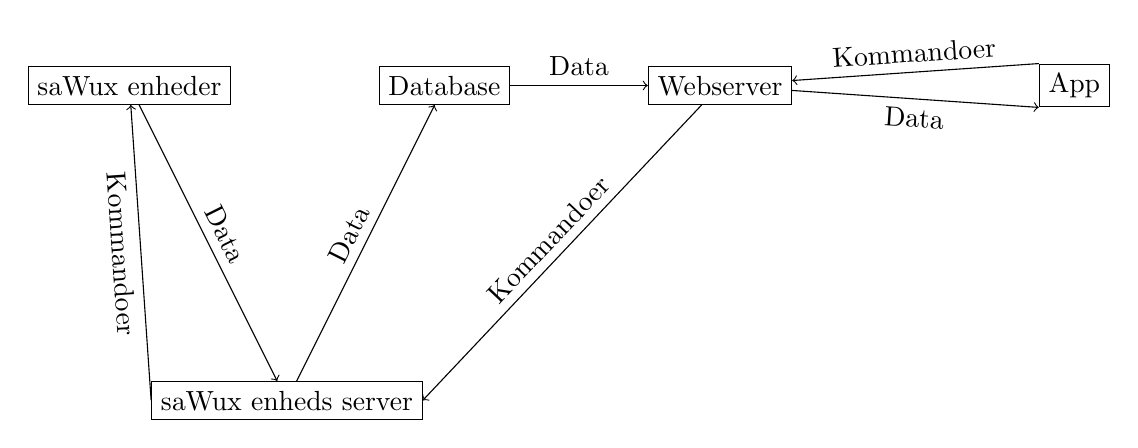
\begin{tikzpicture}
        \node at (0,0) [rectangle,draw] (devices) {saWux enheder};
        \node at (2,-4) [rectangle,draw] (deviceServer) {saWux enheds server};
        \node at (4,0) [rectangle,draw] (database) {Database};
        \node at (7.5,0) [rectangle,draw] (webserver) {Webserver};
        \node at (12,0) [rectangle,draw] (app) {App};

        \draw[->] (deviceServer.west) -- (devices) node [midway, below, sloped] {Kommandoer};
        \draw[->] (webserver)    -- (deviceServer.east) node [midway, above, sloped] {Kommandoer};
        \draw[->] (app.north west)          -- (webserver) node [midway, above, sloped] {Kommandoer};

        \draw[->] (devices)      -- (deviceServer) node [midway, above, sloped] {Data};
        \draw[->] (deviceServer) -- (database) node [midway, above, sloped] {Data};
        \draw[->] (database)     -- (webserver) node [midway, above, sloped] {Data};
        \draw[->] (webserver)    -- (app.south west) node [midway, below, sloped] {Data};
    \end{tikzpicture}
    \caption[Diagram over infrastruktur]{Diagram over \emph{saWux Visualizers} infrastruktur}
    \label{img:teknisk:infra}
\end{figure}
Løsningens infrastruktur, der ses i figur \ref{img:teknisk:infra}, består af en række af elementer. Det første element er sensorer og enheder, leveret af \emph{saWux}. Disse kan modtage kommandoer såsom tænd og sluk fra enhedsserveren. Enhederne sender ligeledes sensordata; blandt andet information om sig selv til enhedsserveren. Enhedsserveren gemmer den modtagne data i en database. Til databasen hører en webserver, der kan sende dataen videre til en app, når appen beder om det. Webserveren kan også modtage kommandoer fra appen og videresender dem til enhedsserveren, som videresender dem til enhederne, der udfører kommandoen. Det sidste element er appen.\\ 

Appen er ansvarlig for at vise enhederne og dataen grafisk, så det er forståeligt for brugeren. Appen er også brugerens måde at interagere med enhederne — ved at lade dem sende kommandoer, såsom tænd og sluk ved at trykke på en knap.

\subsection{Dashboard}
Inden for \emph{saWux Visualizer} er \emph{Dashbordet} er applikationens start- og hovedside. Et interface — hvis hovedformål er at give et generelt overblik over husstandens forbrug. Fra \emph{dashboardet} kan brugeren tilgå alle applikationen delelementer, som er beskrevet nedenfor. Forbruget bliver vist i form af forskellige \emph{cards}, brugerne selv kan tilføje, slette og rykke rundt på. 
\begin{figure}[H]
    \centering
    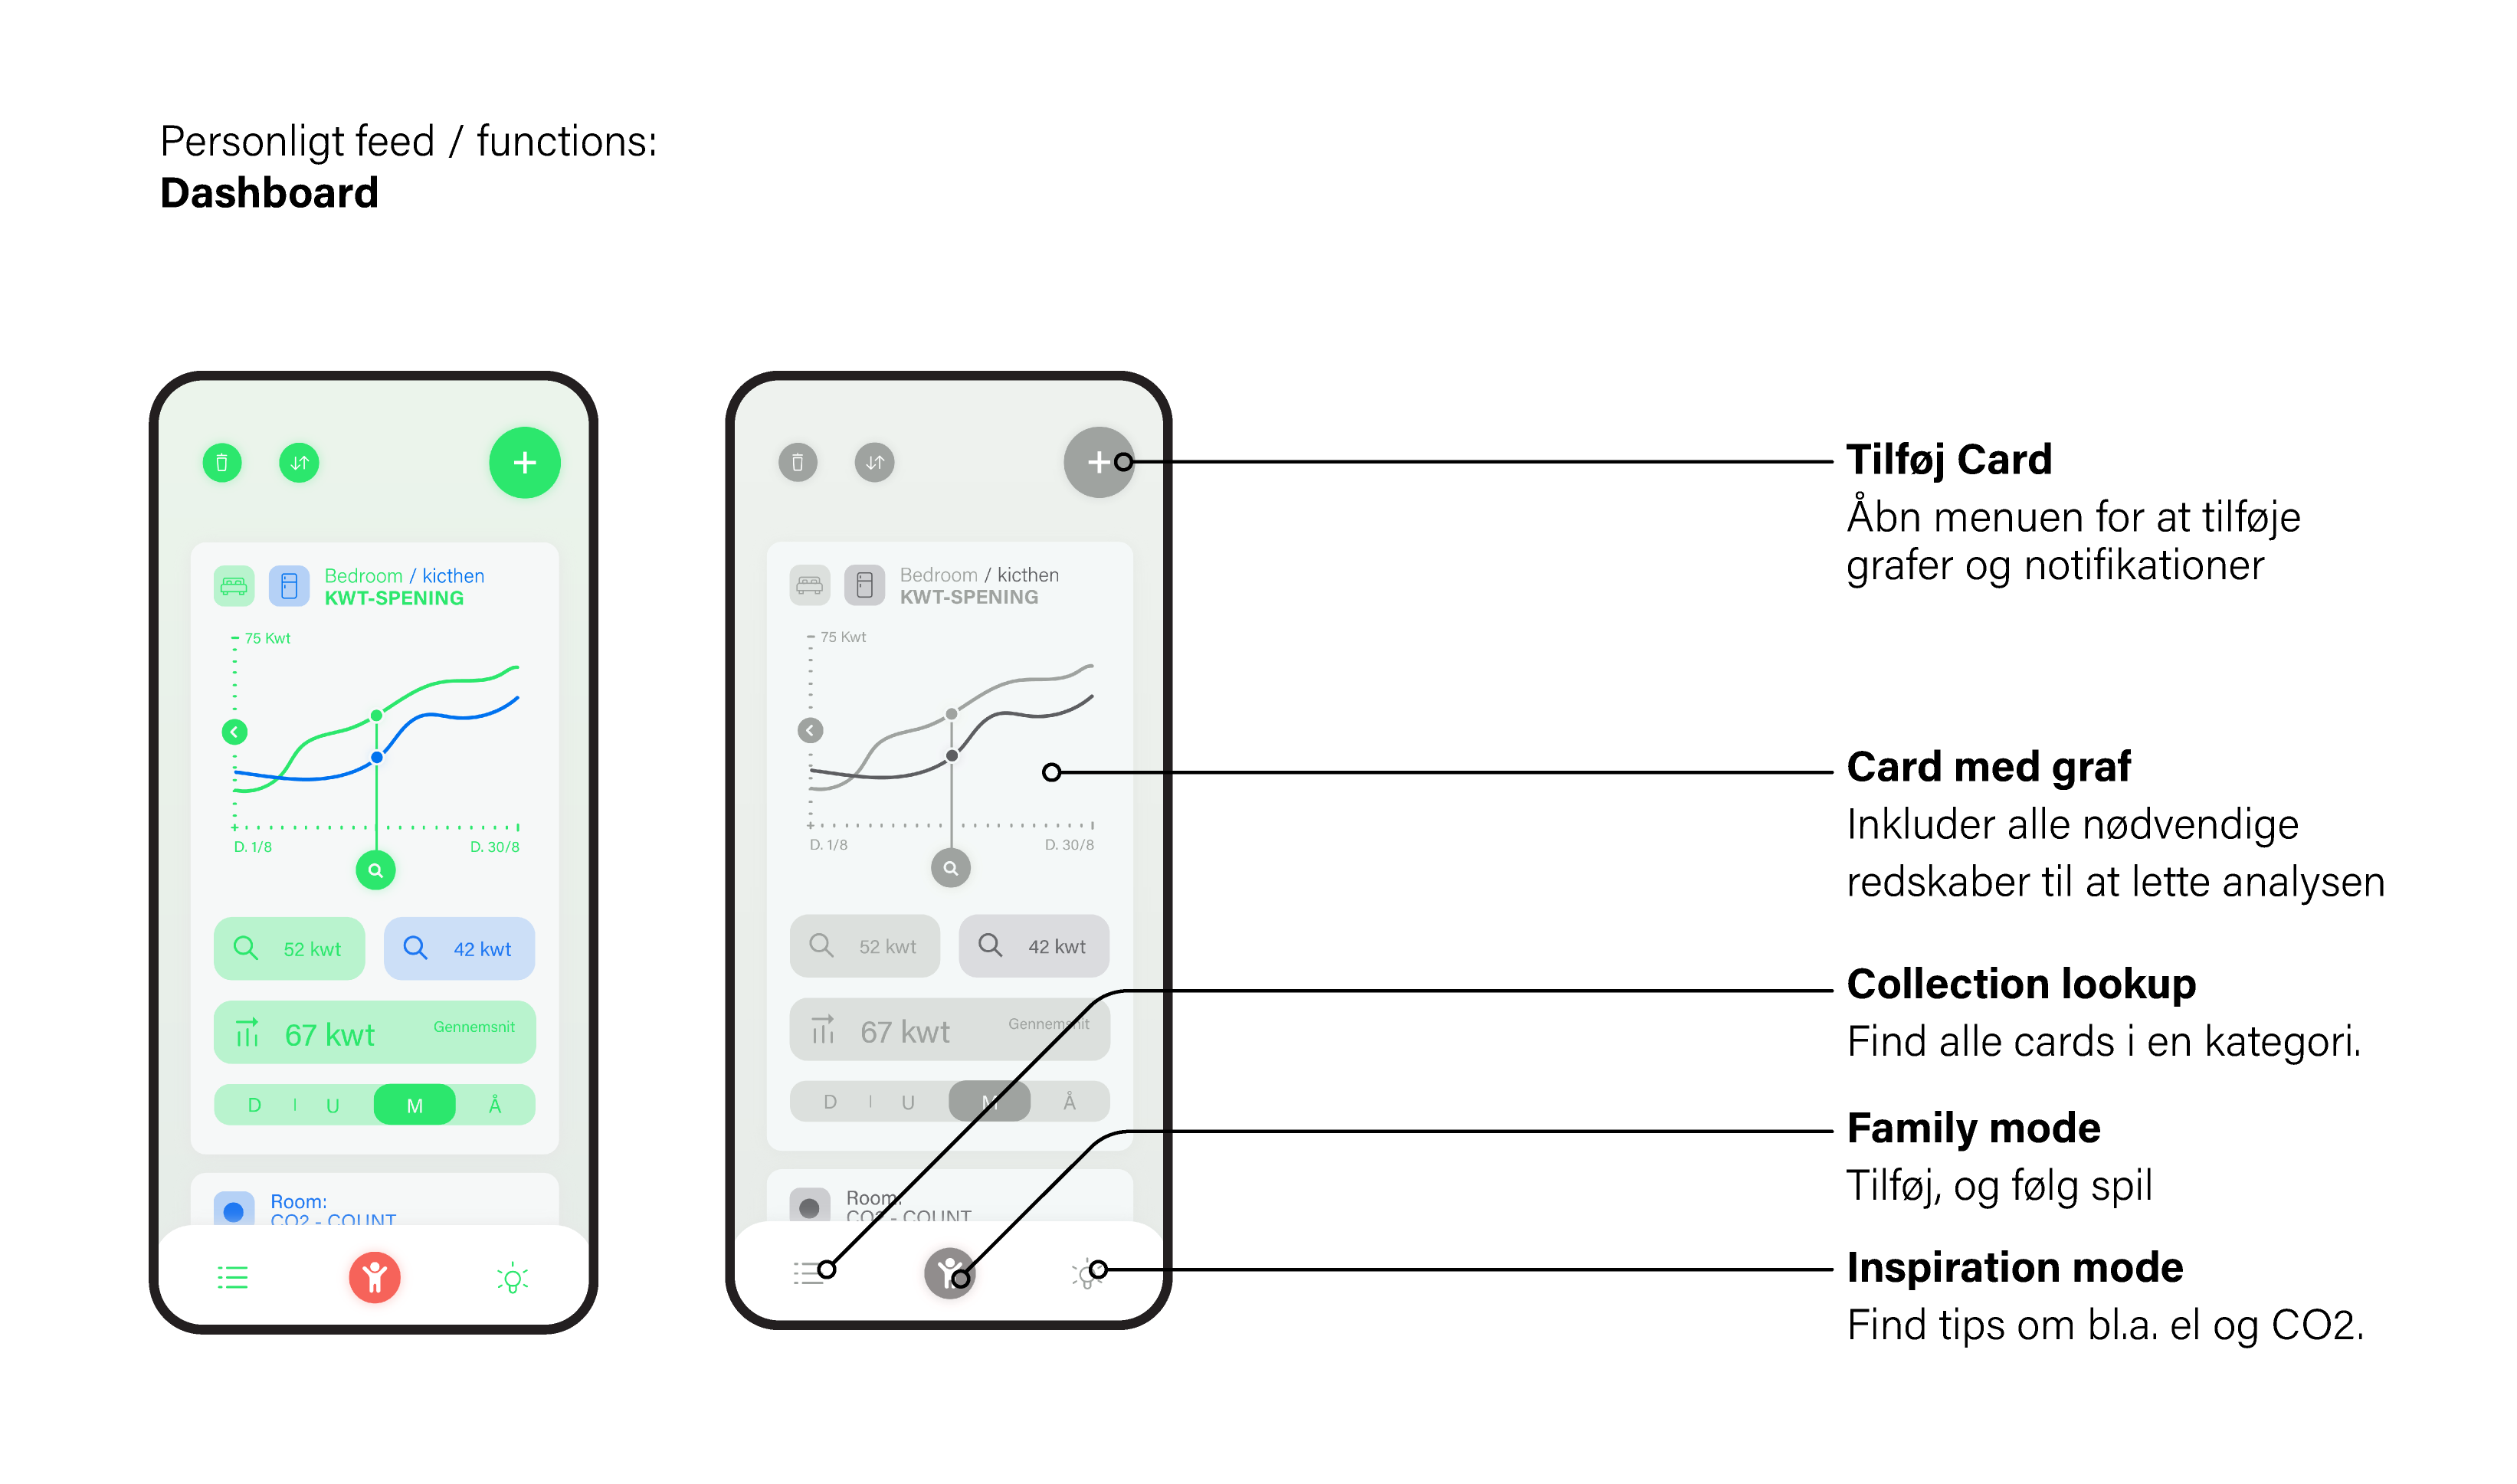
\includegraphics[width=\textwidth]{Images/Main Board.png}
    \caption[\emph{Dashboard} mockup]{Mockup af \emph{saWux Visualizers dashboard}}
    \label{img:teknisk:dashboard}
\end{figure}

\subsection{Cards}
Inden for \emph{saWux Visualizer} er \emph{cards} applikationens visuelle fremstillingsmetode. Formålet med hvert \emph{card} er, at fremstille den indsamlede data på den mest brugervenlige måde. Dette gøres i form af et interaktivt element, der giver brugeren muligheden for at designe hvert \emph{card}, således at det giver den mest optimale individuelle forståelse. Card tilføjes ved at trykke på \emph{+ ikonet} (se figur \ref{img:teknisk:addcard}). Ved tilføjelsen af et \emph{card} gennemløber brugeren en udvælgelsesproces af følgende elementer:
\begin{itemize}
    \item Cardtype — Formålet med dette \emph {card}.
    \item Datatype — Hvilken dataype skal det givne \emph {card} vise.
    \item Graftype — Hvilke graftype skal det givne \emph {card} vise.
    \item Room — Hvilket rum skal det givne \emph {card} indhente data fra.
\end{itemize}
\begin{figure}[H]
    \centering
    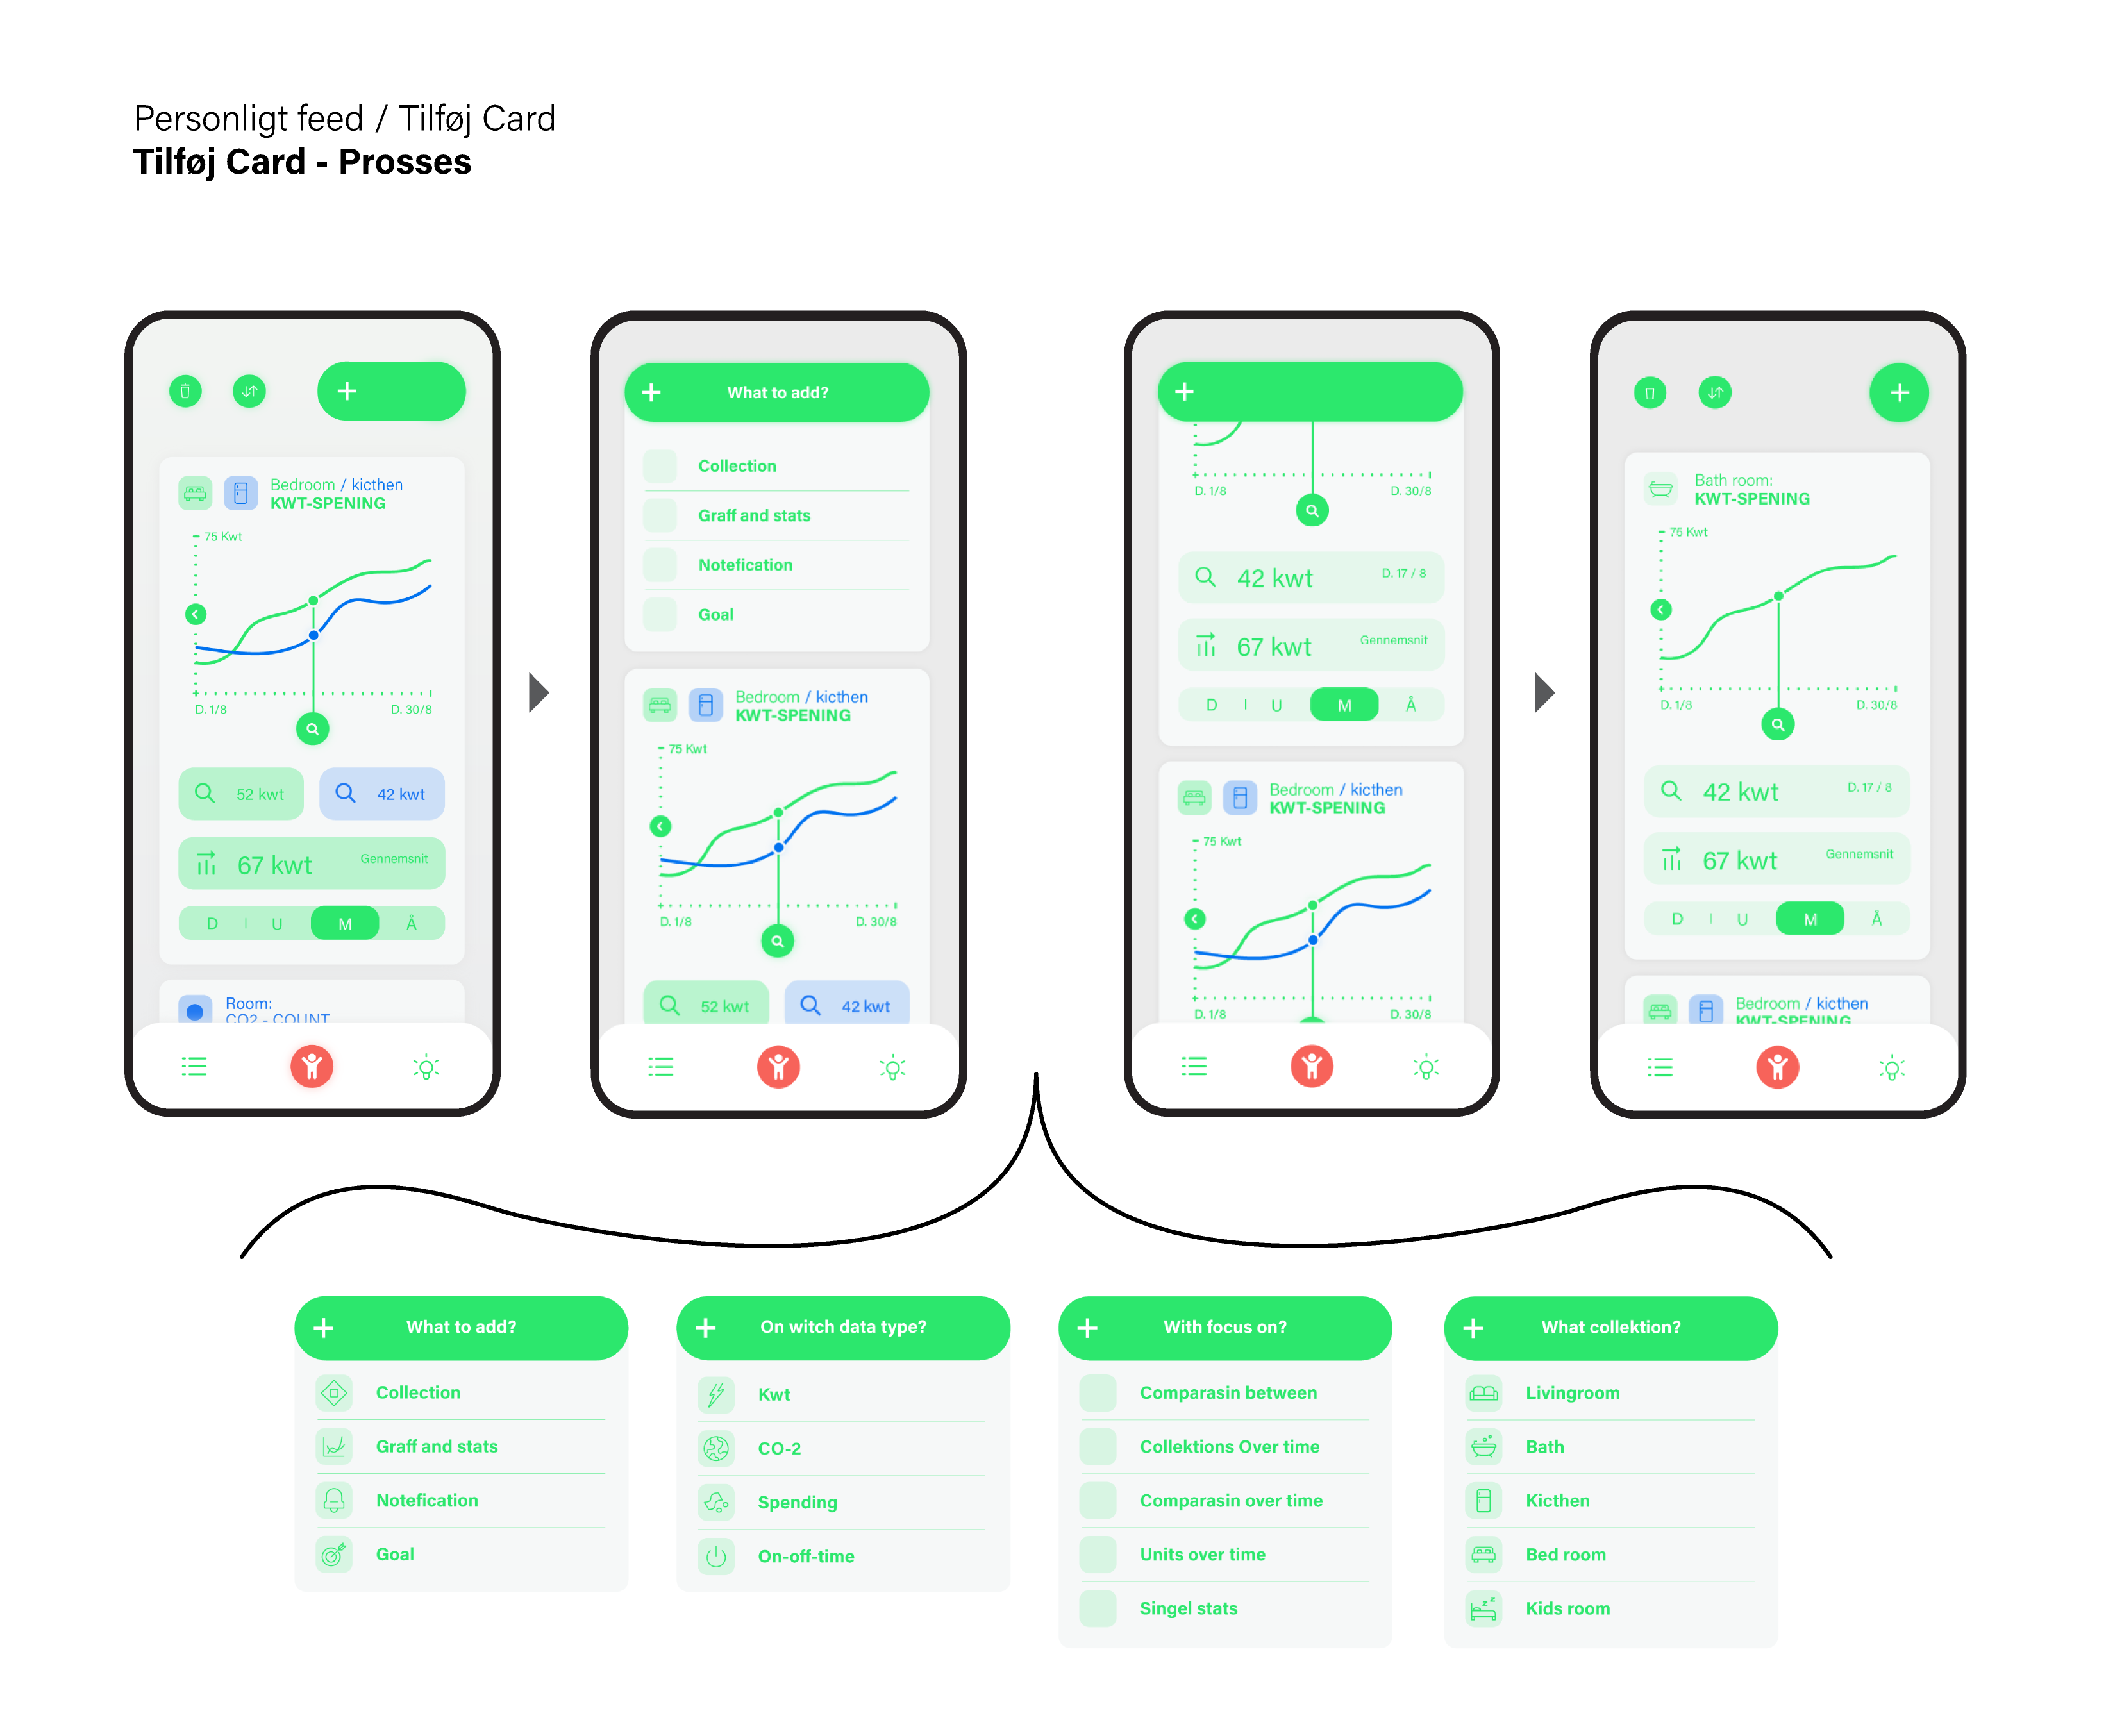
\includegraphics[width=\textwidth]{Images/Add Card.png}
    \caption[Tilføj \emph{card} mockup]{Mockup af funktionen der tilføjer \emph{cards} i appen}
    \label{img:teknisk:addcard}
\end{figure}
På figur \ref{img:teknisk:card} nedenfor ses et eksempel på et \emph{card}, der viser forbruget i \emph{living room}. Dette \emph{card} er opbygget med en interaktiv line-graph, hvor interval af tid findes på $x$-aksen og forbrug af kWh på $y$-aksen. Flytter brugeren på forstørrelsesglas-ikonet, er outputtet det specifikke tal på den givne tid. Desuden illustreres gennemsnitsforbruget for det valgte tidsinterval (D/U/M/Å).
\begin{figure}[H]
    \centering
    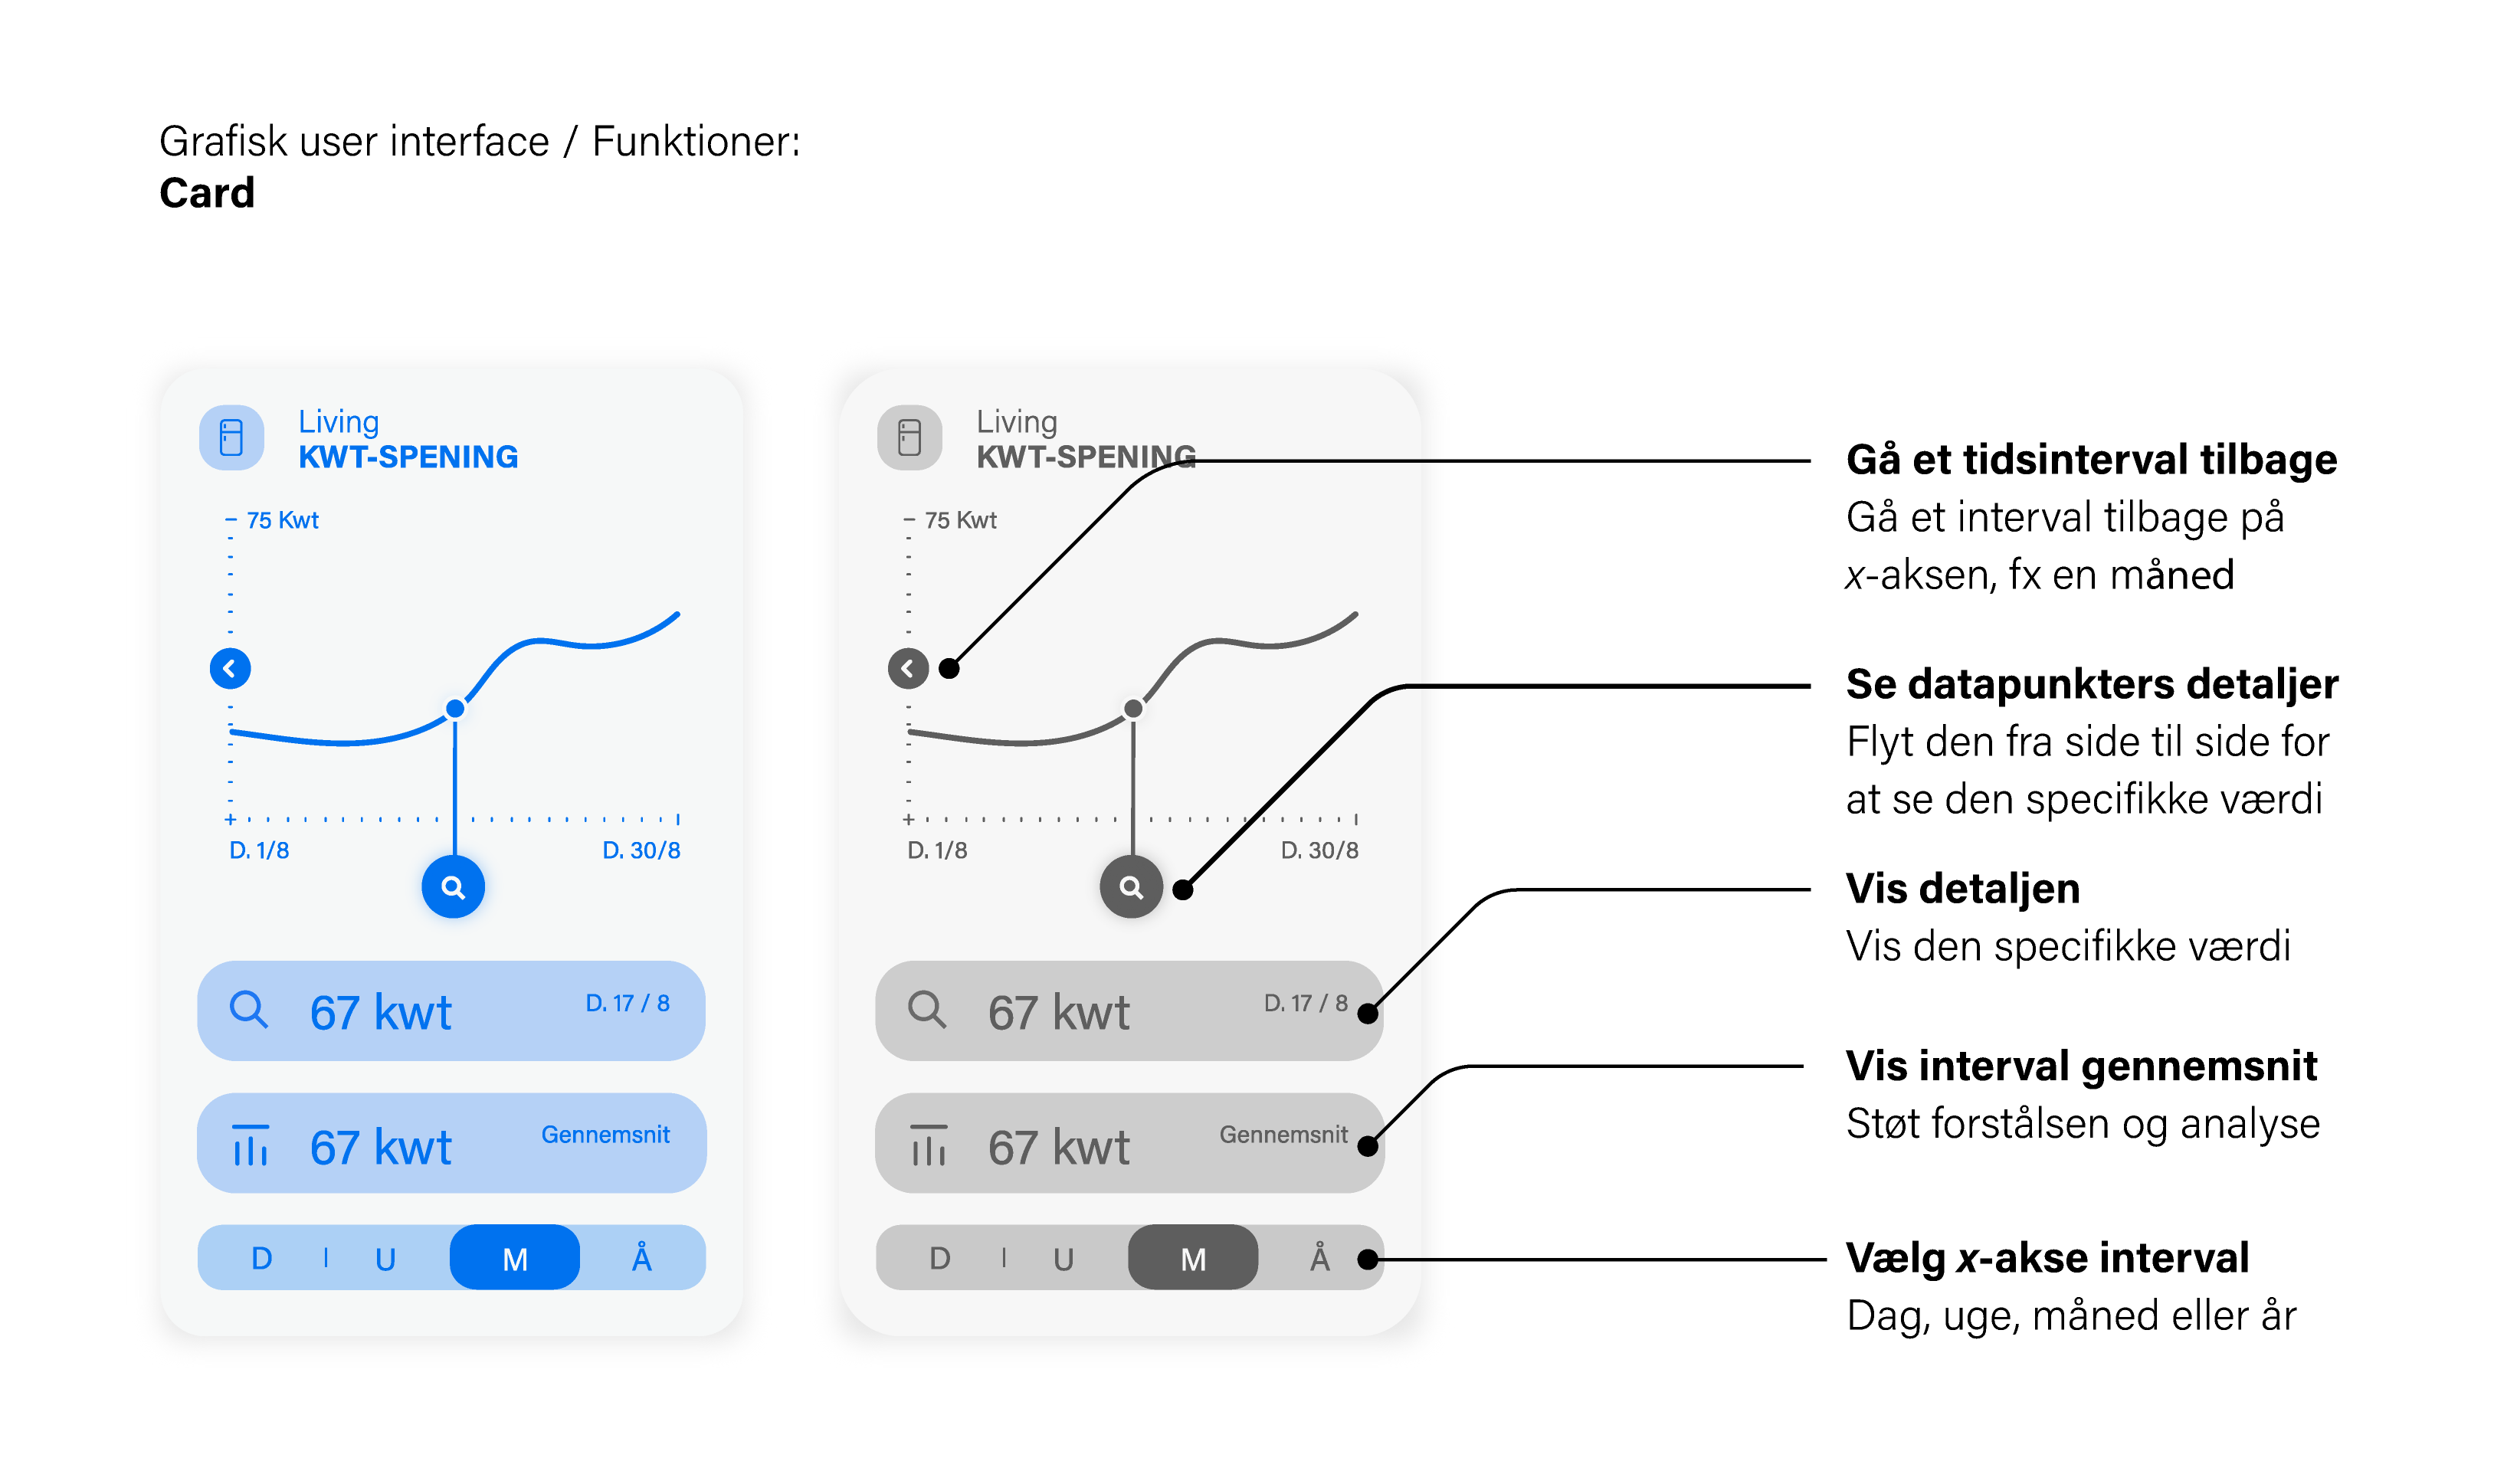
\includegraphics[width=\textwidth]{Images/Main Board - Card.png}
    \caption[\emph{Card} mockup]{Mockup af et specifikt \emph{card}, der viser forbrug af kWh}
    \label{img:teknisk:card}
\end{figure}
\newpage

\subsection{Family Mode}
Inden for \emph{saWux Visualizer} er \emph{Family Mode} et interface, hvor husstanden kan konkurrere i at have den største besparelse. Dette gøres via en spilfunktion, hvor familien kan sammenligne forskellige forbruget i forskellige rum (børneværelset, stuen, ect.). Ved at trykke på \emph{controller +} ikonet øverst i venstre hjørne, får brugeren mulighed for at tilføje forskellige spil og dertil deltagere. Herfra kan familien eksempelvis konkurrere i at bruge færrest kWh, og samtidig se hvem, der klarer sig bedst. Trykker brugeren på \emph{podie-ikonet} øverst til højre, bliver hele historikken af sejre — tidsperioden definerer brugeren selv — visualiseret.
\begin{figure}[H]
    \centering
    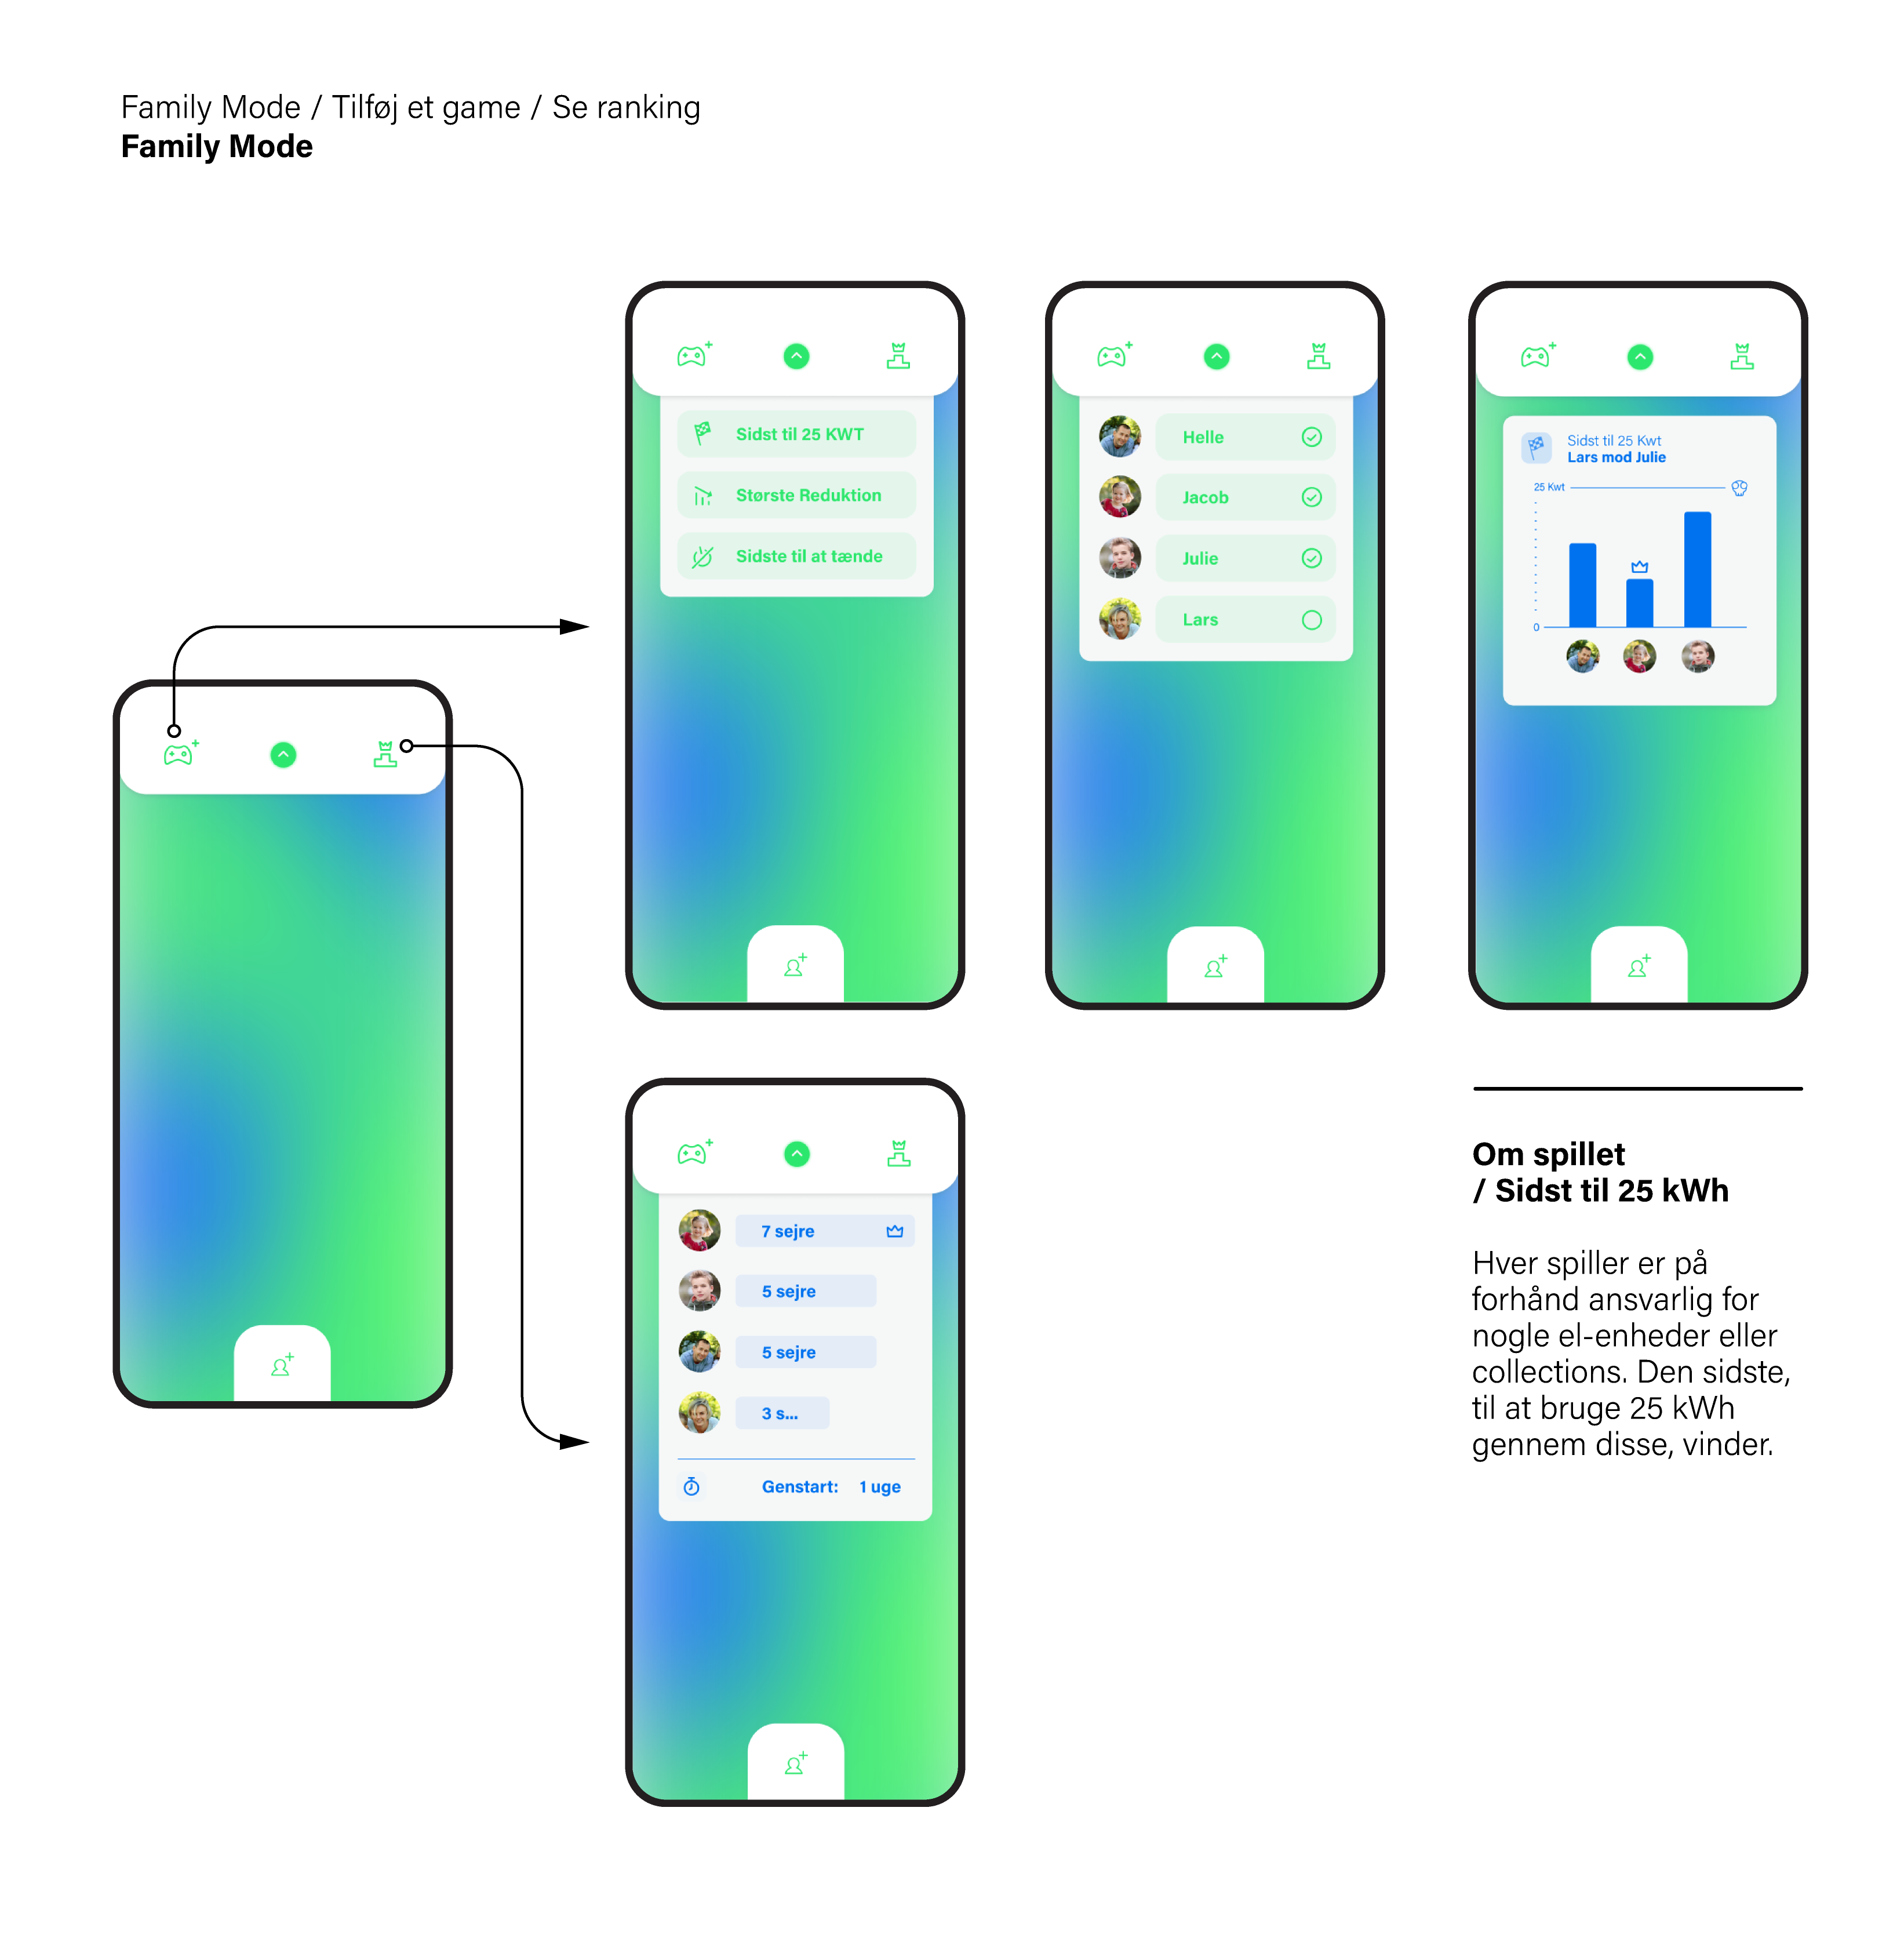
\includegraphics[width=0.8\textwidth]{Images/Kids mode.png}
    \caption[\emph{Family Mode} mockup]{Mockup af funktionen \emph{Family Mode}}
    \label{img:teknisk:kidsmode}
\end{figure}

\subsection{Inspiration Mode}
Inden for \emph{saWux Visualizer} er \emph{Inspiration Mode} applikationens \emph{news feed interface}, hvor brugeren kan tilgå de nyeste informationer om \emph{saWux'} publikationer. Dette interface viser de tre nyeste publiceringer, som illustreres med et \emph{card}, der viser en kategori, en overskrift og et billede. Trykker brugeren på et af de tre \emph{cards}, folder artiklen sig ud og brugeren læser sig til en bedre forståelse af forbrug (el, gasser, etc.), tips og tricks til besparelse samt nye produkter og så videre.
\begin{figure}[H]
    \centering
    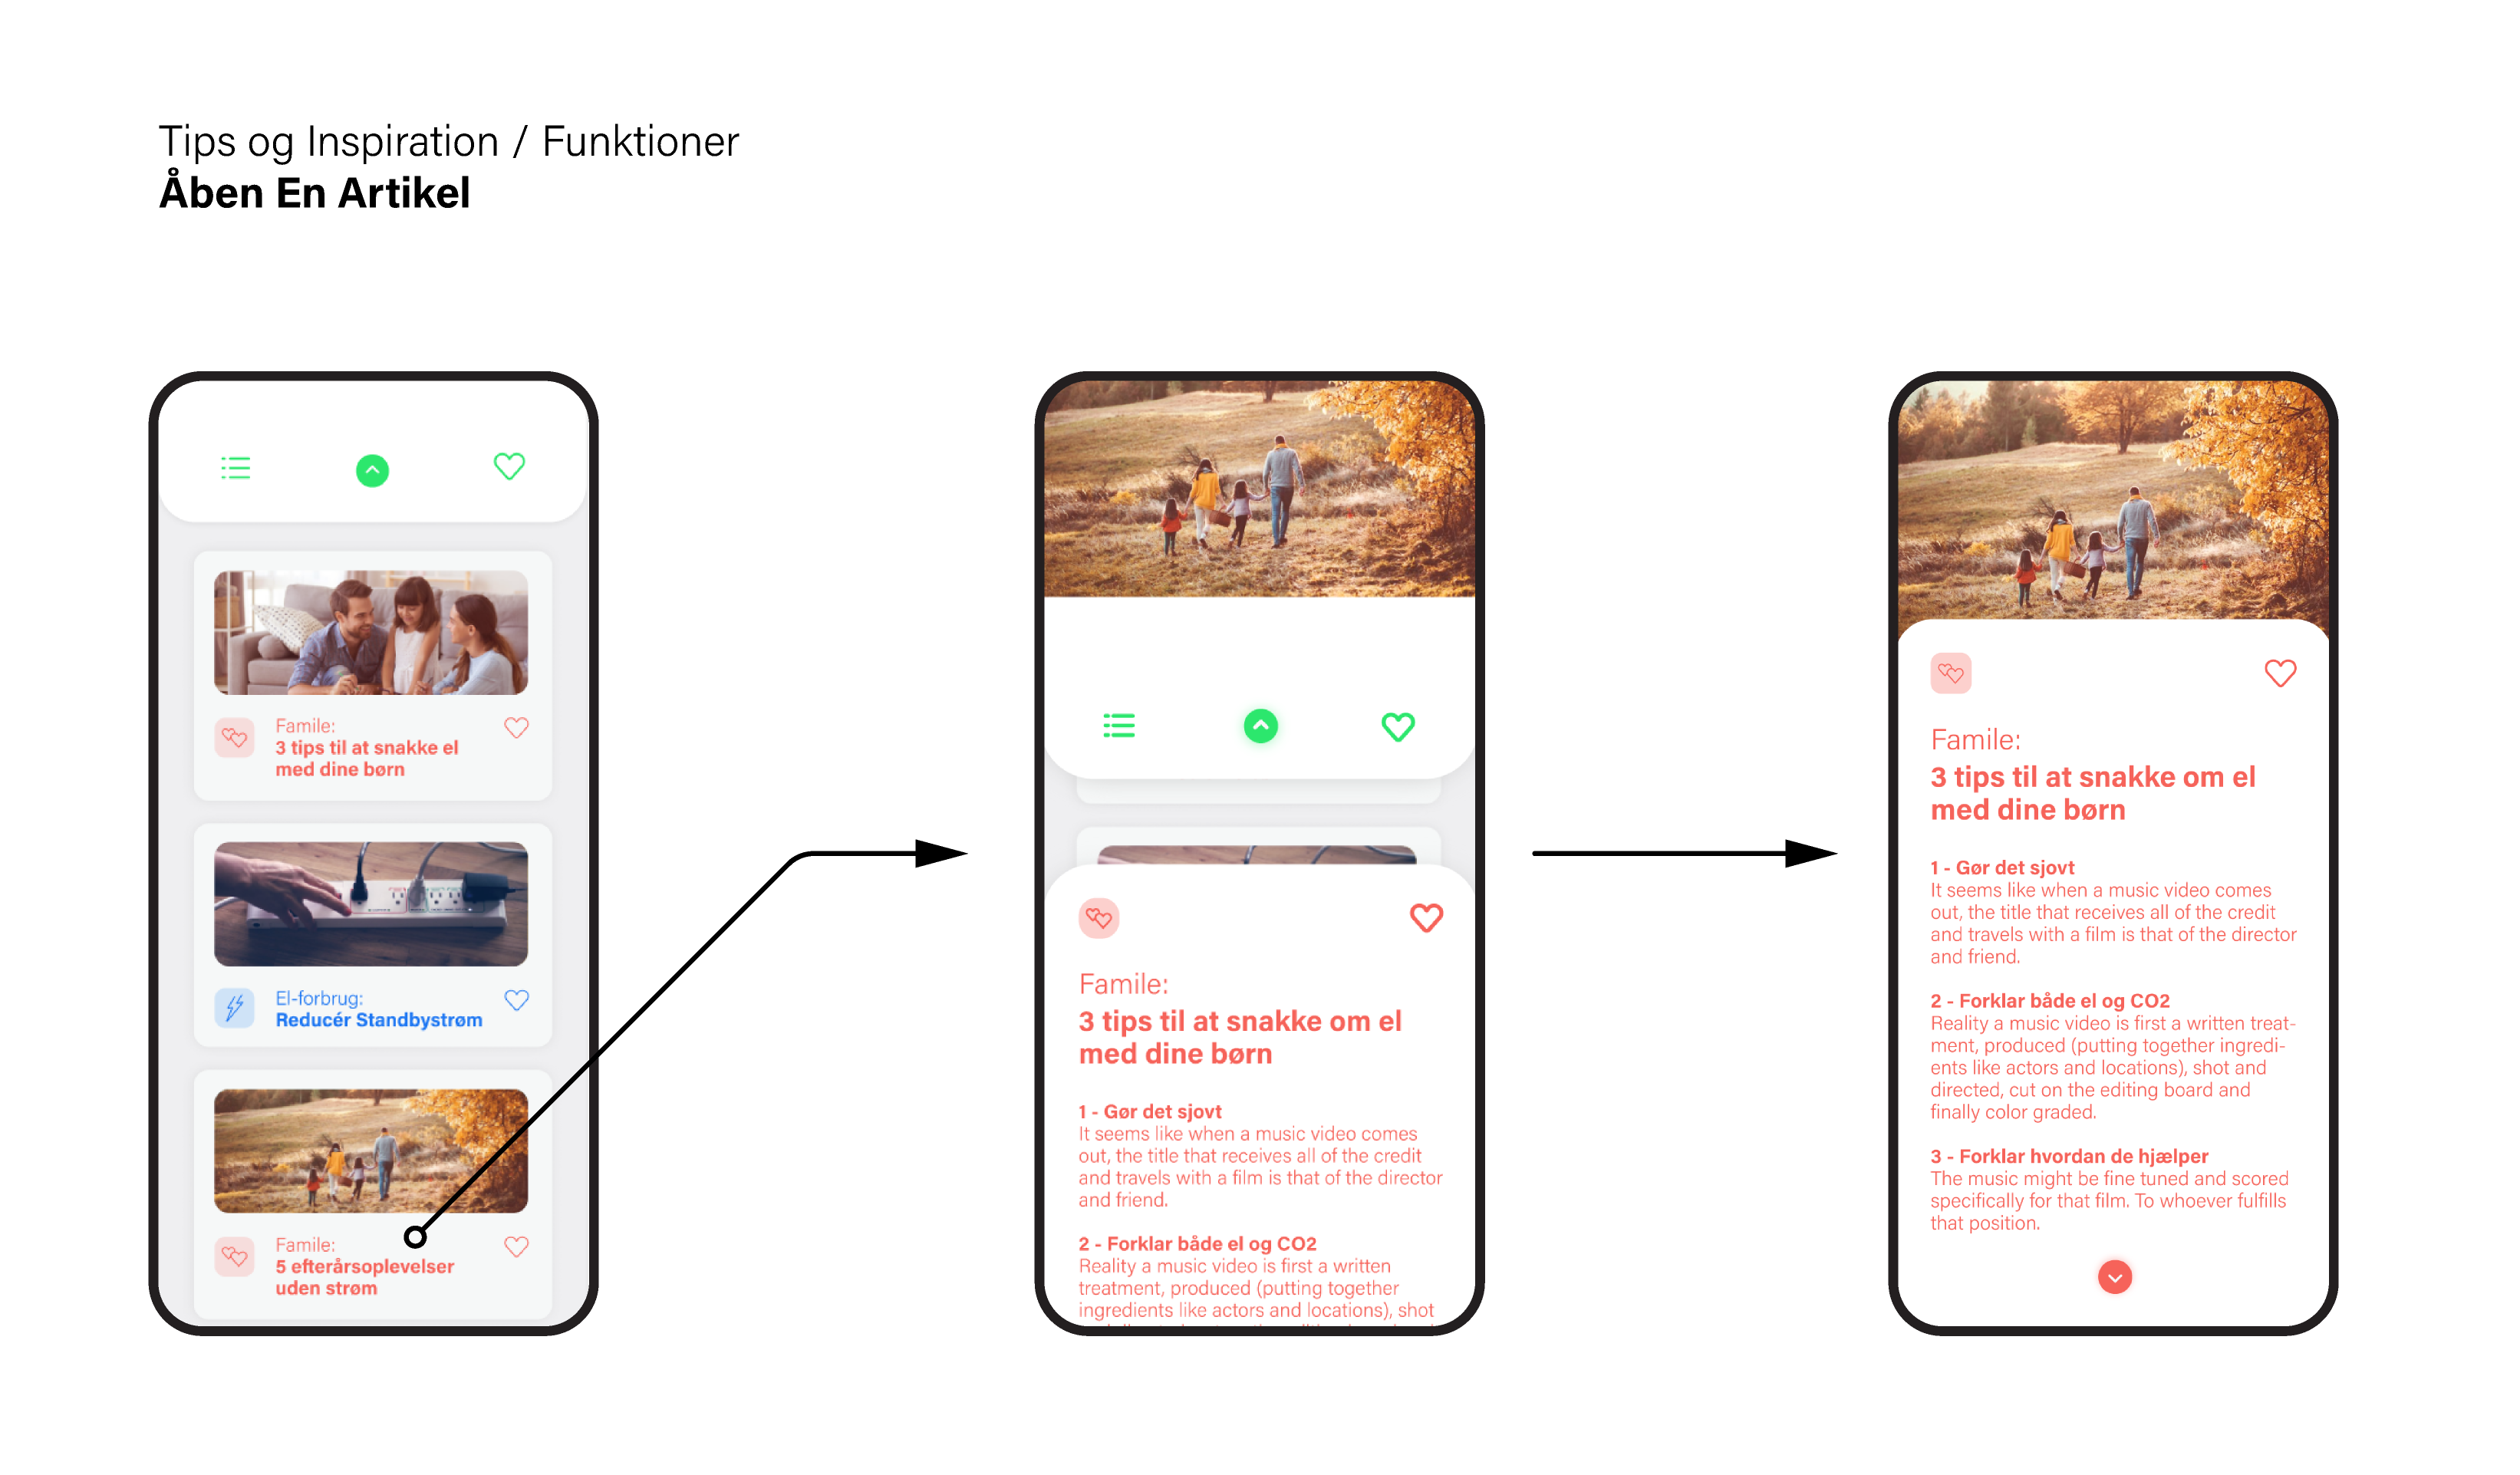
\includegraphics[width=\textwidth]{Images/Open An Article.png}
    \caption[\emph{Inspiration Mode} mockup]{Mockup af \emph{Inspiration Mode}, der viser artikler om blandt andet miljø- og forbrugsbesparelser}
    \label{img:teknisk:article}
\end{figure}
\subsection{Transitions}
Inden for \emph{saWux Visualizer} er \emph{Transitions} måden hvorpå brugeren bevæger sig rundt i applikationen. Overgangen mellem \emph{dashboardet} og applikationens andre interfaces (\emph{Family Mode} og \emph{Inspiration Mode}) sker gennem \emph {navigationsboardet}, som er den menu, der ses nederst på \emph{dashboardet}. Når eksemplevis \emph {Family Mode} er valgt, folder en hvid lokal \emph{bar} med nye funktioner sig ud i toppen af skærmen, således at man kan tilgå og bruge lokale funktioner i den valgte \emph{Mode}. Den miderste knap med en opadvendt pil har samme funktion i alle lokale \emph{Modes}. Funktionen sender brugeren tilbage til \emph {dashboardet}, hvorfra man igen kan tilgå de andre \emph {Modes}.
\begin{figure}[H]
    \centering
    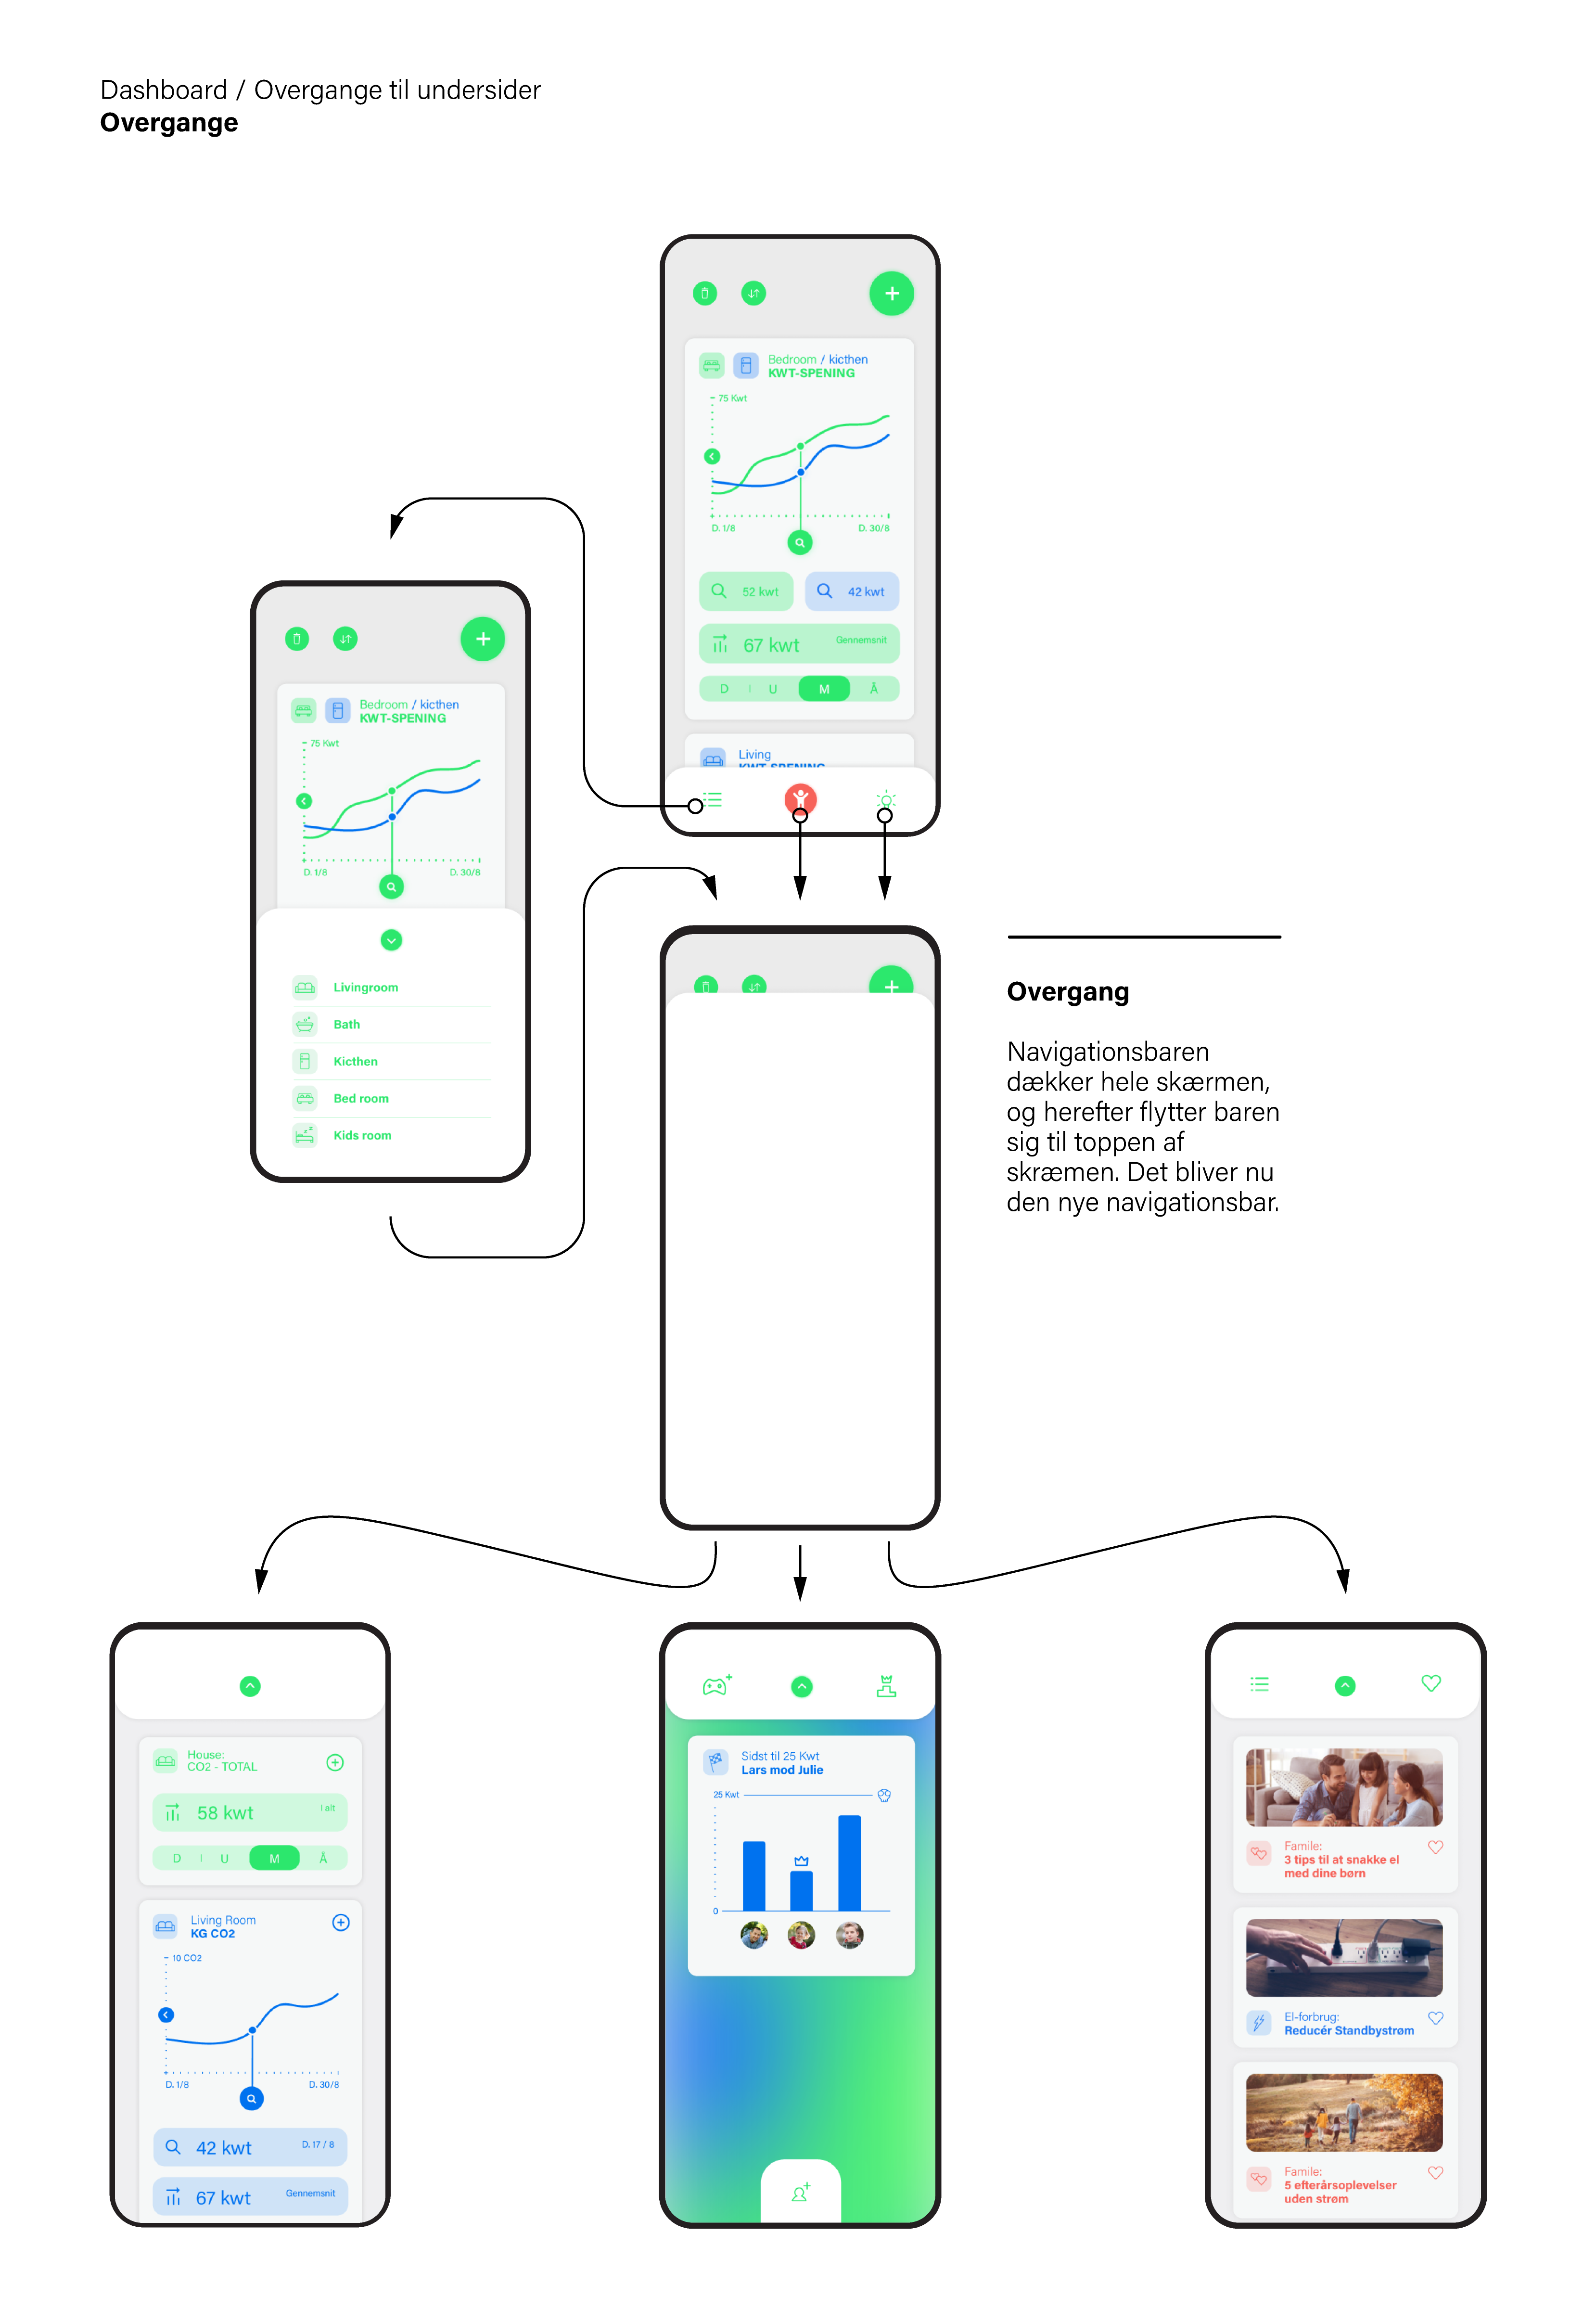
\includegraphics[width=0.9\textwidth]{Images/Transitions.png}
    \caption[\emph{Transitions} mockup]{Mockup af \emph{transitions} eller \emph{overgange} mellem appens forskellig funktioner og sider}
    \label{mockupg:teknisk:transitions}
\end{figure}

\section{Opsummering}
\emph{saWux Visualizer} indsamler data fra \emph{saWux} enheder og giver hurtigt brugeren et overblik over husstandens forbrug. Applikationen er opbygget af interaktive interfaces, der hovedsageligt designes af brugerne selv ved hjælp af forskellige \emph{cards}. Samspillet mellem \emph{saWux Visualizers} delelementer giver brugeren et hurtigt overblik over sine besparelser. Desuden muliggør applikationen at familier kan konkurrere mod hinanden og få inspiration til nye besparelsesmetoder eller andre \emph{saWux} produkter. 
